\documentclass[12pt]{exam}
\usepackage{amsthm}
\usepackage{libertine}
\usepackage[utf8]{inputenc}
\usepackage[margin=1in]{geometry}
\usepackage{amsmath,amssymb}
\usepackage{multicol}
\usepackage[shortlabels]{enumitem}
\usepackage{siunitx}
\usepackage{cancel}
\usepackage{graphicx}
\usepackage{pgfplots}
\usepackage{listings}
\usepackage{tikz}


\pgfplotsset{width=10cm,compat=1.9}
\usepgfplotslibrary{external}
\tikzexternalize\newcommand{\class}{Moderna-Complementaria} % This is the name of the course
\newcommand{\examnum}{Tarea 3} % This is the name of the assignment
\newcommand{\examdate}{10/02/2023} % This is the due date
\newcommand{\timelimit}{}





\begin{document}
\pagestyle{plain}
\thispagestyle{empty}

\noindent
\begin{tabular*}{\textwidth}{l @{\extracolsep{\fill}} r @{\extracolsep{6pt}} l}
\textbf{\class} & \textbf{Name:} & \textit{David Pachon}\\ %Your name here instead, obviously 
\textbf{\examnum} && Sergio Montoya\\
\textbf{\examdate} &&\\
\end{tabular*}\\
\rule[2ex]{\textwidth}{2pt}
% ---

\begin{enumerate}
  \item \begin{figure}[h]
      \centering
      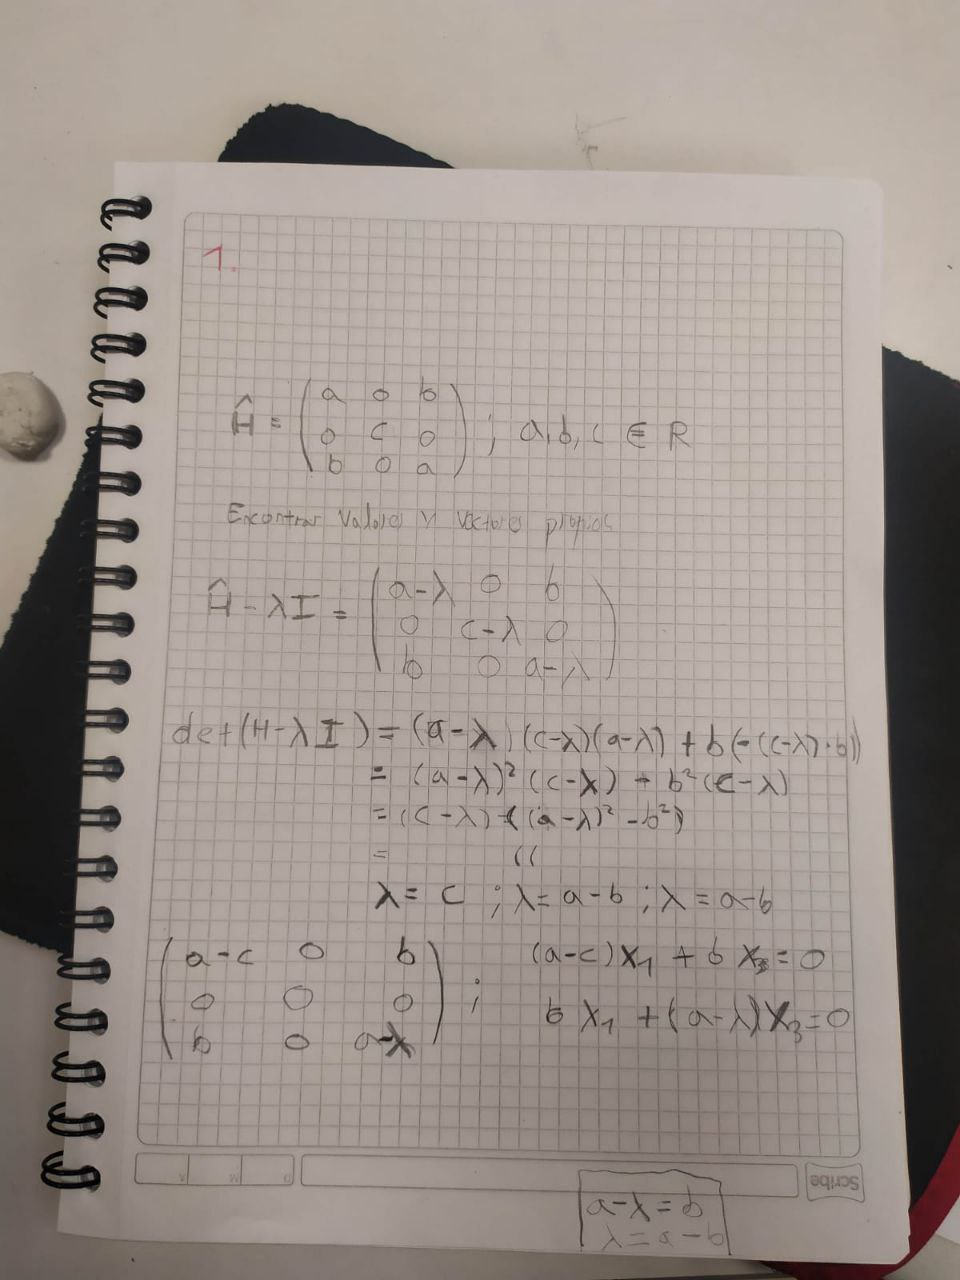
\includegraphics[scale=0.5]{Moderna_14_04.jpg}
    \end{figure}
  \item Para comenzar hagamos recuento del teorema de Ehrenfest el cual dice
    \begin{equation}
      \frac{d<A>}{dt}=\frac{i}{h}\left<[\hat{H},\hat{A}] \right>+\left<\frac{\partial\hat{A}}{\partial t}\right>
    .\end{equation}
    Y dado que partimos desde \[
    \frac{d<xp>}{dt}
    .\] Ahora bien, tomemos también en cuenta que
    \begin{align}
      [\hat{A},\hat{B}\hat{C}] &= [\hat{A},\hat{B}]\hat{C} + [\hat{A},\hat{C}]\hat{B}\\
      [f(\hat{A}),\hat{B}] &= \frac{\partial f}{\partial A} [\hat{A},\hat{B}]\\
      \hat{K} = \frac{\hat{P}}{2m}\\
      \hat{p} = \frac{-\hbar}{i}\frac{\partial}{\partial x}
  \end{align}
  
  Ahora bien, con todo esto partamos el desarrollo
  \begin{align*}
    \frac{d<xp>}{dt}&=\frac{i}{\hbar}\left<[\hat{H},xp]\right>+\left<\frac{\partial xp}{\partial t}\right>\\
		    &=\frac{i}{\hbar}\left<[\hat{H},x]p+[\hat{H},p]x\right>+\left<p\frac{\partial x}{\partial t} + x\frac{\partial p}{\partial t}\right>\\
    \frac{\partial p}{\partial t} &= 0\\
    \frac{\partial x}{\partial t} &= V\\
				  &= \frac{i}{\hbar}\left<[\hat{H},x]p+[\hat{H},p]x\right>+\left<pV\right>\\
				  &= \frac{i}{\hbar}\left<[\hat{H},x]p+[\hat{H},p]x\right>-\frac{i}{\hbar}\left<\frac{\partial v}{\partial x}\right>\\
    [\hat{H},x]f &= \hat{H}\hat{x}-\hat{x}\hat{H}\\
		 &= \left( \frac{\hat{p}^2}{2m} + \hat{V} \right) \hat{x}f - \hat{x}\left( \frac{\hat{p}^2}{2m}+\hat{v} \right)f\\
		 &=\left(\frac{1}{2m}\left( -i\hbar\frac{\partial}{\partial x} \right)^2\hat{x}f+ \hat{V}\hat{x}f \right)  - \hat{x}\left( \frac{1}{2m}\left( -i\hbar \frac{\partial}{\partial x}\right)f + \hat{V}f \right)\\
		 &=\left(\frac{1}{2m}\left( \hbar^2\frac{\partial^2}{\partial x^2} \right)\hat{x}f+ \hat{V}\hat{x}f \right)  - \hat{x}\left( \frac{1}{2m}\left( \hbar^2 \frac{\partial^2}{\partial x^2}\right)f + \hat{V}f \right)\\
  .\end{align*}
\end{enumerate}



\end{document}
